\documentclass[tikz,border=3pt]{standalone}
\usepackage[utf8]{inputenc}
\usepackage[T1]{fontenc}
\usepackage{lmodern}
\renewcommand{\familydefault}{\sfdefault}
\usepackage{sansmath}\sansmath
\usepackage{chemfig}
\usepackage{pgfplots}\pgfplotsset{compat=1.18,/pgf/number format/use comma,/pgf/number format/1000 sep={.}}
\usetikzlibrary{arrows.meta,calc,positioning,decorations.pathmorphing,patterns}
% paleta del sitio
\definecolor{nar}{HTML}{E8680C}\definecolor{narc}{HTML}{FFB35C}\definecolor{hielo}{HTML}{FFF3E8}
\definecolor{tinta}{HTML}{1D1D1F}\definecolor{gris}{HTML}{6E6E73}\definecolor{lila}{HTML}{7C5CF0}
\definecolor{azul}{HTML}{2F6FD6}\definecolor{menta}{HTML}{17A673}\definecolor{coral}{HTML}{E8342A}
\begin{document}
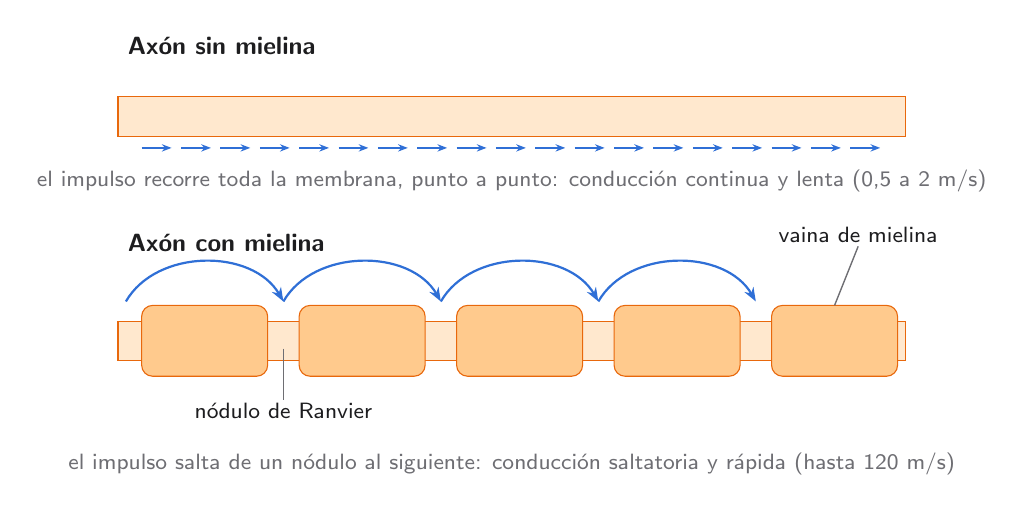
\begin{tikzpicture}[font=\small]
% axon sin mielina
\node[anchor=west,font=\small\bfseries,text=tinta] at (0,3.75) {Axón sin mielina};
\fill[narc!30,draw=nar] (0,2.6) rectangle (10,3.1);
\foreach \x in {0.3,0.8,...,9.3}{\draw[-{Stealth[length=3.5pt]},azul,thick] (\x,2.45) -- ++(0.38,0);}
\node[anchor=north,text=gris,font=\footnotesize] at (5,2.3) {el impulso recorre toda la membrana, punto a punto: conducción continua y lenta (0,5 a 2 m/s)};
% axon con mielina
\node[anchor=west,font=\small\bfseries,text=tinta] at (0,1.25) {Axón con mielina};
\fill[narc!30,draw=nar] (0,-0.25) rectangle (10,0.25);
\foreach \x in {0.3,2.3,4.3,6.3,8.3}{\draw[nar,fill=narc!70,rounded corners=4pt] (\x,-0.45) rectangle ++(1.6,0.9);}
\foreach \x in {0.1,2.1,4.1,6.1}{\draw[-{Stealth[length=5pt]},azul,thick] (\x,0.5) to[out=60,in=120] (\x+2,0.5);}
\begin{scope}[gris,line width=0.5pt]
\draw (9.1,0.45) -- (9.4,1.2) node[anchor=south,text=tinta,font=\footnotesize,inner sep=1pt] {vaina de mielina};
\draw (2.1,-0.1) -- (2.1,-0.75) node[anchor=north,text=tinta,font=\footnotesize,inner sep=1pt] {nódulo de Ranvier};
\end{scope}
\node[anchor=north,text=gris,font=\footnotesize] at (5,-1.3) {el impulso salta de un nódulo al siguiente: conducción saltatoria y rápida (hasta 120 m/s)};
\end{tikzpicture}
\end{document}
